%%%%%%%%%%%%%%%%%%%%%%%%%%%%%%%%%%%%%%%%%%%%%%%%%%%%%%%%%%%%
%%  This Beamer template was created by Cameron Bracken.
%%  Anyone can freely use or modify it for any purpose
%%  without attribution.
%%
%%  Last Modified: January 9, 2009
%%

\documentclass[xcolor=x11names,compress,framenumber]{beamer}

%% General document %%%%%%%%%%%%%%%%%%%%%%%%%%%%%%%%%%

\usepackage{textpos}
\usepackage{graphicx}
\usepackage[utf8]{inputenc}
\usepackage[brazil]{babel}
\usepackage{tikz}
\usepackage{pgf}
\usepackage{amsmath}
\usepackage{epstopdf}
\usepackage{multimedia}
\graphicspath{{Figuras/}}

%%%%%%%%%%%%%%%%%%%%%%%%%%%%%%%%%%%%%%%%%%%%%%%%%%%%%
%% colors

\definecolor{lettercolor}{rgb}{0, 0.2,  0.5}
\definecolor{BgColor}{rgb}{ 0.98823529,  0.98823529,  0.58039216}

\usetikzlibrary{arrows,shapes,automata,petri,positioning,patterns}
\tikzset{
	place/.style={
		circle,
		thick,
		draw=lettercolor!75,
		fill=white!20,
		minimum size=6mm
	},
	tokens/.style={
		colored tokens = lettercolor
	},
	transition/.style={
		rectangle,
		thick,
		fill=lettercolor,
		minimum width=8mm,
		inner ysep=2pt
	},
	vtransition/.style={
		rectangle,
		thick,
		fill=lettercolor,
		minimum height=8mm,
		inner xsep=2pt
	},
	block/.style={
		rectangle,
		thick,
		draw=lettercolor!75,
		fill=white!20,
		minimum height=1cm,
		minimum width=3cm,
		text centered
	},
	arrow/.style={
		draw=lettercolor!75,
		thick,
		->,
		>=stealth
	},
	cercle/.style={
		circle,
		thick,
		draw=lettercolor!75,
		fill=white!20,
		text centered
	},
} 

\newcommand{\colvector}[3]{\left[ \begin{array}{c}
		#1 \\ #2 \\ #3
	\end{array}\right]}
\newcommand{\doublecolvector}[6]{\left[ \begin{array}{cc}
		#1 & #4 \\ #2 & #5 \\ #3 & #6
	\end{array}\right]}

%% Beamer Layout %%%%%%%%%%%%%%%%%%%%%%%%%%%%%%%%%%
%Se quiser que apareça as subseções no layout, fazer subsection=true

\useoutertheme[subsection=true,shadow,footline=authorinstitutetitle]{miniframes}


\useinnertheme{default}
\usefonttheme{serif}
\usepackage{palatino}

\setbeamerfont{title like}{shape=\scshape}
\setbeamerfont{frametitle}{shape=\scshape}

\setbeamercolor*{lower separation line head}{bg=DeepSkyBlue4}
%\setbeamercolor*{normal text}{fg=black,bg=white}
\setbeamercolor*{alerted text}{fg=red!100}
\setbeamercolor*{example text}{fg=black}
\setbeamercolor*{structure}{fg=lettercolor}%fg=lettercolor
\setbeamercolor*{normal text}{fg=lettercolor,bg=BgColor!10}
\setbeamercolor*{frametitle}{fg=lettercolor}

\setbeamercolor*{palette tertiary}{fg=black,bg=black!10}
\setbeamercolor*{palette quaternary}{fg=black,bg=black!10}
\setbeamercolor*{block title}{fg=lettercolor,bg=white}
\setbeamercolor*{block body}{fg=lettercolor,bg=white}
\setbeamertemplate{blocks}[rounded][shadow=true]
\addtobeamertemplate{block begin}{\pgfsetfillopacity{0.7}}{\pgfsetfillopacity{1}}%0.7 / 1
\addtobeamertemplate{block alerted begin}{\pgfsetfillopacity{0.5}}{\pgfsetfillopacity{1}}%0.5/1

\newcommand{\vecx}{\underline{x}}

\renewcommand{\(}{\begin{columns}}
\renewcommand{\)}{\end{columns}}
\newcommand{\<}[1]{\begin{column}{#1}}
\renewcommand{\>}{\end{column}}
\newcommand{\ls}[1]{ \left \{ {#1}  \right \} }

\newcommand{\bulletpoint}[1]{\begin{itemize}
		\item #1
\end{itemize}}

%%%%%%%%%%%%%%%%%%%%%%%%%%%%%%%%%%%%%%%%%%%%%%%%%%



%\AtBeginSection[]
%{
%  \begin{frame}[plain]{Sumario da apresentação}
%    \tableofcontents[currentsection]
%  \end{frame}
%}


%%%%%%%%%%%%%%%%%%%%%    BACKGROUND %%%%%%%%%%%%%%%%%%%%%%

%%%% podem colocar a transparencia com \pgfsetfillopacity{0.75} entre 0 e 1.

\logo{\pgfputat{\pgfxy(-6,-0.24)}{\pgfbox[center,base]{\pgfsetfillopacity{0.09}{
\includegraphics[width=1.1\textwidth]{pres_fondo1.png}}}}}

%% Rodapé %%%%%%%%%%%%%%%%%%%%%%%%%%%%%%%%%%%%%%%%%%%%%%%%

\title{Um modelo temporizado para identificação e detecção de falhas de sistemas a eventos discretos \hspace{2.3cm} \insertframenumber/\inserttotalframenumber}
\author{Ryan Pitanga Cleto de Souza}
\institute{DEE-UFRJ}

%% Rodapé %%%%%%%%%%%%%%%%%%%%%%%%%%%%%%%%%%%%%%%%%%%%%%%%



% \defbeamertemplate*{footline}{shadow theme}
% {%
%  \leavevmode%
%  \hbox{\begin{beamercolorbox}[wd=.25\paperwidth,ht=2.5ex,dp=1.125ex,leftskip=.3cm plus1fil,rightskip=.3cm]{author in head/foot}%
%    \usebeamerfont{author in head/foot}\insertframenumber\,/\,\inserttotalframenumber\hfill\insertshortauthor
%  \end{beamercolorbox}%
%  \begin{beamercolorbox}[wd=.75\paperwidth,ht=2.5ex,dp=1.125ex,leftskip=.3cm,rightskip=.3cm plus1fil]{title in head/foot}%
%    \usebeamerfont{title in head/foot}\insertshorttitle%
%  \end{beamercolorbox}}%
%  \vskip0pt%
% }

\begin{document}



%%%%%%%%%%%%%%%%%%%%%%%%%%%%%%%%%%%%%%%%%%%%%%%%%%%%%%
% Página de título
%%%%%%%%%%%%%%%%%%%%%%%%%%%%%%%%%%%%%%%%%%%%%%%%%%%%%%


{
\usebackgroundtemplate{%

  \makebox[0pt][t]{
\includegraphics[width=1.185\hsize]{pres_title1.pdf}}}

\begin{frame}[plain]
\vspace*{8mm}
\title{Um modelo temporizado para identificação e detecção de falhas de sistemas a eventos discretos}
\author{\vspace{-.3cm} Ryan Pitanga Cleto de Souza
	}
\date{\vspace{1cm} 21 de março de 2019}
\institute[DEE/UFRJ]{Email: ryanpitanga@poli.ufrj.br}
\titlepage
\end{frame}
}


%%%%%%%%%%%%%%%%%%%%%%%%%%%%%%%%%%%%%%%%%%%%%%%%%%%%%
% BANCA
%%%%%%%%%%%%%%%%%%%%%%%%%%%%%%%%%%%%%%%%%%%%%%%%%%%%%

\begin{frame}{Membros da Banca}


\begin{itemize}
 \item Prof. Marcos Vicente de Brito Moreira (Orientador) \\
 \item Prof. Lilian Kawakami Carvalho \\
 \item Prof. Gustavo da Silva Viana \\
\end{itemize}

\end{frame}



%%%%%%%%%%%%%%%%%%%%%%%%%%%%%%%%%%%%%%%%%%%%%%%%%%%%%%
% SUMARIO
%%%%%%%%%%%%%%%%%%%%%%%%%%%%%%%%%%%%%%%%%%%%%%%%%%%%%



\begin{frame}{Sumário}
\tableofcontents
\end{frame}



%%%%%%%%%%%%%%%%%%%%%%%%%%%%%%%%%%%%%%%%%%%%%%%%%%%%%
%%% Secao Introducao e outras
%%%%%%%%%%%%%%%%%%%%%%%%%%%%%%%%%%%%%%%%%%%%%%%%%%%%%

% Exemplo de citação:
%\begin{quote}
%Um autômato é um dispositivo capaz de representar linguagens
%\end{quote}

\section{Introdução}

% O comando \pause serve para não mostrar o que vem após ele no mesmo slide durante a apresentação.

\begin{frame}{Sistemas a eventos discretos (SED)}
\begin{block}{}
	\begin{itemize}
		\item Conjunto discreto de estados
		\item Evolução através de ocorrências de eventos
	\end{itemize}
\end{block}
\begin{block}{Aplicações}
	\begin{itemize}
		\item Computação
		\item Transportes
		\item Sistemas industriais
	\end{itemize}
\end{block}
\end{frame}

\begin{frame}{Diagnóstico de falhas}
\begin{block}{}
\begin{itemize}
\item Parte importante da pesquisa em SED foi dedicada ao diagnóstico de falhas
\end{itemize}
\end{block}
\begin{block}{Características da abordagem tradicional}
\begin{itemize}
	\item Modelagem analítica completa do sistema
	\item Conhecimento dos comportamentos pós-falha
	\item Determina-se facilmente qual falha ocorreu
\end{itemize}
\end{block}
\end{frame}

%% Colocar exemplo de diagnosticador Sampath?

\begin{frame}{Diagnóstico de falhas}
\begin{block}{}
\bulletpoint{Contudo, a utilização desses métodos em sistemas industriais é difícil}
\end{block}
\begin{block}{Desvantagens para sistemas de grande porte}
\begin{itemize}
\item Modelo complexo
\item Não leva em conta consequências não previstas para as falhas 
\item Necessidade de um engenheiro que conheça os formalismos necessários à modelagem
\end{itemize}
\end{block}
\end{frame}

\begin{frame}{Modelagem por identificação}
\begin{block}{}
\bulletpoint{Para contornar os problemas apresentados, foi proposta uma abordagem por identificação}  
\end{block}
\begin{block}{Características da modelagem por identificação}
\begin{itemize}
\item Não há necessidade de qualquer conhecimento prévio sobre o sistema
\item Modelo construído a partir de sinais do controlador obtidos do comportamento livre de falhas 
\item Procedimento automatizado
\end{itemize}
\end{block} 
\end{frame}

\begin{frame}{Modelagem por identificação}
\begin{block}{}
	\bulletpoint{Uso do modelo identificado na detecção de falhas}
	\begin{figure}[]
		\centering
		\begin{tikzpicture}[node distance = 2cm]
		\node (system) [block] {Sistema};
		\node (model) [block,below of = system] {Modelo};
		\node (entrada) [xshift = -3cm,yshift = -1cm] {Entradas};
		\node (comparador) [cercle,xshift=2cm,yshift=-1cm]{};
		\node (diagnosis) [block,right of = comparador,xshift=0.5cm]{Detecção de falhas};
		
		\draw [arrow] (entrada) |- (system);
		\draw [arrow] (entrada) |- (model);
		\draw [arrow] (system) -| (comparador) node [anchor=south,xshift=0.5cm,yshift=1cm]{Saídas};
		\draw [arrow] (model) -| (comparador) node [anchor=north,xshift=0.5cm,yshift=-1cm]{Saídas};
		\draw [arrow] (comparador) -- (diagnosis) {};
		
		\draw (2+0.18*1.41/2,-1-0.18*1.41/2) -- (2-0.18*1.41/2,-1+0.18*1.41/2);
		\draw (2-0.18*1.41/2,-1-0.18*1.41/2) -- (2+0.18*1.41/2,-1+0.18*1.41/2);
		
		\end{tikzpicture}
		%\caption{Esquema mostrando como funciona a detecção de falhas baseada em modelo.}
		\label{fig:esquema detection}
	\end{figure}	
\end{block}

\end{frame}

\section[Fundamentos]{Fundamentos teóricos}

%\begin{frame}{Fundamentos}
%\begin{block}{}
%	\begin{itemize}
%		\item Todo SED tem um conjunto $ \Sigma $ de eventos associado
%	\end{itemize}
%\end{block}
%\begin{block}{Linguagens}
%	\begin{itemize}
%		\item É um conjunto de sequências de eventos pertencendo a $ \Sigma $
%		\item Podem ser usadas para modelar o comportamento de SEDs
%	\end{itemize}	
%\end{block}
%\begin{block}{Exemplo}
%	\begin{equation*}
%		\Sigma = \left\lbrace a,b,c\right\rbrace 
%	\end{equation*}
%	\begin{equation*}
%		L = \left\lbrace ab,acb,aab,abac,cab\right\rbrace 
%	\end{equation*}
%\end{block}
%\end{frame}
%
%\begin{frame}{Autômato}
%%\bulletpoint{Autômato}
%\begin{block}{}
%	\begin{figure}
%		\centering
%		\begin{tikzpicture}[shorten >=1pt,node distance=2cm,on grid,auto] 
%		\node[state,accepting] (x)   {$x$}; 
%		\node[state,accepting] (z) [below right=of x] {$z$};
%		\node[state] (y) [above right=of z] {$y$}; 
%		\node[state,accepting] (z) [below right=of x] {$z$}; 
%		\path[->] 
%		(x) edge  node [swap] {$ g $} (z)
%		edge  [loop above] node {$ a $} ()
%		(y) edge  node [swap]  {$ a $} (x)
%		edge [loop above] node {$ b $} ()
%		(z) edge  node [swap] {$ a,g $} (y) 
%		edge [loop below] node {$ b $} ();
%		\draw[->] (-1,0) -- (-0.5,0);
%		\end{tikzpicture}
%		%\caption{Diagrama de transição de estados do autômato do exemplo \ref{ex:automato}.}
%		\label{fig:exemplo automato}
%	\end{figure}
%	\begin{equation*}
%	\begin{split}
%	f(x,a) &= x \\
%	f(x,g) &= z \\
%	\end{split}
%	\quad\quad
%	\begin{split}
%	f(y,a) &= x\\
%	f(y,b) &= y\\
%	\end{split}
%	\quad\quad
%	\begin{split}
%	f(z,a) &= y\\
%	f(z,b) &= z\\
%	\end{split}
%	\quad\quad
%	\begin{split}
%	f(z,g) &= y \\
%	\\
%	\end{split}
%	\end{equation*}
%\end{block}
%\end{frame}

\begin{frame}{Autômato temporizado com guardas}
%\bulletpoint{}
\begin{block}{}
\begin{figure}
\centering
\begin{tikzpicture}[shorten >=1pt,node distance=3cm,on grid,auto] 
\node[state] (x0)   {$0$}; 
\node[state] (x1) [right=of x0] {$1$}; 
\node[state] (x2) [right=of x1] {$2$}; 
\node[state] (x3) [right=of x2] {$3$};
\node [below=of x2,yshift=2.2cm] {$ c_1 < 1 $};
%(x2) node[anchor=north]{$ c_1 < 1 $}; 
\path[->] 
(x0) edge  node {$ -;a;c_1 $} (x1)
(x1) edge  node  {\footnotesize$ 0<c_1<1;a;c_1 $} (x2)
edge [loop below] node {$ c_1\geq 1;a;c_1 $} ()
(x2) edge node {$ -;b;- $} (x3)
;
\draw[->] (-1,0) -- (-0.5,0);
\end{tikzpicture}
%\caption{Autômato temporizado do exemplo \ref{ex:automato temporizado}.}
\label{fig:exemplo automato temporizado}
\end{figure}
\begin{itemize}
	\item Uma restrição sobre o tempo de ocorrência do evento é associada a cada transição
	\item Cada transição é rotulada por (guarda;evento;reset) 
\end{itemize}
\end{block}
\end{frame}

%\begin{frame}{Rede de Petri}
%%\bulletpoint{}
%\begin{block}{}
%\begin{equation*}
%\begin{split}
%&P = \left\lbrace p_1,p_2,p_3\right\rbrace \\
%&T = \left\lbrace t_1\right\rbrace \\
%&\textbf{x}_0 = [1\:\:0\:\:2]^T
%\end{split}
%\quad\quad
%\begin{split}
%&Pre(p_1,t_1) = 1 \\
%&Pre(p_2,t_1) = 0 \\
%&Pre(p_3,t_1) = 1 \\
%\end{split}
%\quad\quad
%\begin{split}
%&Post(t_1,p_1) = 0 \\
%&Post(t_1,p_2) = 2 \\
%&Post(t_1,p_3) = 0
%\end{split}
%\end{equation*}
%\begin{figure}[h!]
%\centering
%\begin{tikzpicture}[node distance=1.5cm,>=stealth',bend angle=45,auto]
%\node [place,tokens=1,label=above: $ p_1 $] (p1) {};
%\node [vtransition] (t1) [right of = p1,label=above:$ t_1 $] {};
%\node [place,label=above: $ p_2 $] (p2)[right of = t1] {};
%\node [place,label = below: $ p_3 $,colored tokens={lettercolor,lettercolor}] (p3)[below of = p1] {};	
%\path[->]
%(t1) edge[pre]  node {} (p1)
%(t1) edge[post] node {$ 2 $} (p2)
%(t1) edge[pre] node {} (p3);
%\draw (1.55/2+2.70/2,0.1) -- (1.55/2+2.70/2,-0.1);
%\end{tikzpicture}
%%\caption{Rede de Petri do exemplo \ref{ex:rede de Petri marcada}.}
%\label{fig:rede de Petri marcada}
%\end{figure}
%%\begin{equation*}
%%\textbf{x}_0 = [1\:\:0\:\:2]^T
%%\end{equation*}
%\end{block}
%\end{frame}

\begin{frame}{Rede de Petri}
\begin{block}{}
\bulletpoint{Exemplo (sistema de fila)}
\begin{figure}
\centering
\begin{tikzpicture}[node distance=1.5cm,>=stealth',bend angle=45,auto]
\node [vtransition] (t1) [label=below:$ t_1 $,label=above:$ a $] {};
\node [place,label=above: $ Q $,label=below: $ p_1 $] (Q)[right of = t1] {};
\node [vtransition] (t2) [right of = Q,label=below:$ t_2 $,label=above:$ s $] {};
\node [place,label=above: $ B $,label=below: $ p_2 $] (B)[right of = t2]{};
\node [vtransition] (t3) [right of = B,label=below:$ t_3 $,label=above:$ d $] {};
\node [place,tokens=1,label=above: $ I $,label=right: $ p_3 $,colored tokens=lettercolor] (I)[above of = B]{};

\path[->]
(t1) edge[post] node {} (Q)
(t2) edge[pre] node {} (Q)
(t2) edge[post] node {} (B)
(t2) edge[pre] node {} (I)
(t3) edge[pre] node {} (B)
(t3) edge[post] node {} (I)
;
\end{tikzpicture}
%\caption{Rede de Petri rotulada do exemplo \ref{ex:rede de Petri rotulada}.}
\label{fig:rede de Petri rotulada}
\end{figure}
\end{block}
\end{frame}
%
\begin{frame}{Rede de Petri interpretada para controle}
\begin{block}{}
\begin{itemize}
\item Extensão da definição de rede de Petri
\item Modelagem do controle de um processo industrial
\end{itemize}
\end{block}
\begin{block}{}
	\begin{itemize}
		\item Ações associadas a lugares
		\begin{itemize}
			\item Contínuas
			\item Impulsionais
		\end{itemize}
	\item Receptividades ou atrasos associados às transições
	\begin{itemize}
		\item Não-temporizadas
		\item Temporizadas
	\end{itemize}
	\end{itemize}
\end{block}
\end{frame}

\begin{frame}{Rede de Petri interpretada para controle}
	\begin{block}{Transições (não-temporizadas x temporizadas)}
		\begin{figure}
			\begin{center}
				\begin{tabular}{cc}
					\begin{tikzpicture}[node distance=1.5cm,>=stealth',bend angle=45,auto]
					\node [vtransition] (t1) [label=below:$ t_j $,label=above:$ \sigma_j\text{,}c_j $] {};
					\node [place] (Q)[left of = t1] {};
					\node [place] (Q1)[right of = t1] {};
					
					\path[->]
					(t1) edge[post] node {} (Q1)
					(t1) edge[pre] node {} (Q)
					;
					\end{tikzpicture}
					\quad\quad\quad
					\begin{tikzpicture}[node distance=1.5cm,>=stealth',bend angle=45,auto]
					\node [vtransition] (t1) [label=below:$ d_j $,label=above:$ t_j $] {};
					\node [place] (Q)[left of = t1] {};
					\node [place] (Q1)[right of = t1] {};
					
					\path[->]
					(t1) edge[post] node {} (Q1)
					(t1) edge[pre] node {} (Q)
					;
					\end{tikzpicture}
				\end{tabular}
				%\caption{Exemplo de transição com evento e condição associados.}
				%\label{fig:tj sigmaj cj}
			\end{center}
		\end{figure}
	\end{block}	
	\begin{block}{Ações ($ A_i $: contínua, $ B_i $: impulsional)}
		\begin{figure}
			\begin{center}
				\begin{tikzpicture}[node distance=1.5cm,>=stealth',bend angle=45,auto]
				\node [vtransition] (t1) [] {};
				\node [place] (Q)[right of = t1,label=below:$ p_i $,label=above:$ A_i\text{,}B_i^* $] {};
				\node [vtransition] (t2) [right of = Q] {};
				
				\path[->]
				(t1) edge[post] node {} (Q)
				(t2) edge[pre] node {} (Q)
				;
				\end{tikzpicture}
				%\caption{Exemplo de transição com evento e condição associados.}
				%\label{fig:tj sigmaj cj}
			\end{center}
		\end{figure}
	\end{block}	
\end{frame}

\begin{frame}{Rede de Petri interpretada para controle}
\begin{block}{Exemplo (acendimento de uma lâmpada)}
\begin{figure}
\centering
\begin{tikzpicture}[node distance=1.5cm,>=stealth',bend angle=45,auto]
\node [place,tokens=1,colored tokens=lettercolor] (p1)[] {};
\node [transition] (t1) [below of = p1,label=right:$ \uparrow\! b $] {};
\node [place] (p2)[below of = t1,label=right:Lâmpada acesa] {};
\node [transition] (t2) [below of = p2,label=right:$ t\text{=}10s $] {};

\path[->]
(t1) edge[pre] node {} (p1)
(t1) edge[post] node {} (p2)
(t2) edge[pre] node {} (p2)
;
\draw[->] (t2) to[out=-160,in=160] (p1) ;
\end{tikzpicture}
%\caption{RPIC do exemplo \ref{ex:rpic lampada}}
\label{fig:ex rpic}
\end{figure}
\end{block}
\end{frame}

\begin{frame}{Falhas}

	\begin{block}{}
		\emph{É uma condição física que faz um dispositivo, um componente, ou um elemento a não funcionar da forma desejada.} 
	\end{block}
	
	\begin{block}{Exemplos}
		\begin{itemize}
			\item curto-circuito
			\item fio solto
			\item conexão intermitente
		\end{itemize}
	\end{block}

\end{frame}

\begin{frame}{Falhas}
	
	\begin{block}{Diagnóstico}
		\begin{enumerate}
			\vspace{0.5cm}
			\item \textit{Detecção de falhas} é a decisão entre duas situações: algo está errado ou tudo está normal
			\vspace{0.5cm}
			\item \textit{Isolamento da falha} é a determinação de onde a falha ocorreu (qual sensor, qual equipamento, etc.)
		\end{enumerate}	
	\end{block}

	\begin{block}{}
		Neste trabalho, o interesse será a modelagem por identificação com vistas à \textbf{detecção de falhas}.
	\end{block}
	
\end{frame}
	
\section{Modelagem por identificação}

\begin{frame}{Modelagem por identificação}
	\begin{block}{}
		\begin{itemize}
			\item Os sinais do controlador são coletados com o sistema funcionando livre de falha
			
			\item Um modelo é construído a partir dos dados coletados, de forma a reproduzir os comportamentos observados
			
			\item O processo de aquisição de sinais deve durar tempo suficiente para que o modelo gerado possa representar o sistema satisfatoriamente
		\end{itemize}
	
		
	\end{block}
\end{frame}

\begin{frame}{Procedimento de aquisição}
\begin{block}{}
	\begin{figure}
		\centering
		\begin{tikzpicture}[node distance = 2cm]
		\node (plant) [block] {Planta};
		\node (actuators) [block,above of = plant, xshift = -2cm, yshift = -0.75cm] {Atuadores};
		\node (sensors) [block,above of = plant, xshift = 2cm, yshift = -0.75cm] {Sensores};
		\node (controller) [block,above of = plant, yshift = 1cm] {Controlador};
		\draw [arrow] (plant) -| (sensors);
		\draw [arrow] (actuators) |- (plant);
		\draw [arrow] (sensors) |- (controller);
		\draw [arrow] (controller) -| (actuators);
		\filldraw[fill=lettercolor!75,draw=lettercolor!75] (2,2.8) circle (0.05cm);
		\filldraw[fill=lettercolor!75,draw=lettercolor!75] (-2,2.2) circle (0.05cm);
		\draw [arrow] (2,2.8) -- (3.8,2.8) node [anchor=west]{sinais de entrada};
		\draw [arrow] (-2,2.2) -- (3.8,2.2) node [anchor=west]{sinais de saída};		
		\end{tikzpicture}
%		\caption{Esquema mostrando a comunicação entre os componentes envolvidos no sistema.}
%		\label{fig:esquema sistema}
	\end{figure}
\end{block}
\end{frame}

\begin{frame}{Procedimento de aquisição}

\begin{block}{Vetor I/O}
\begin{equation*}
u_j:=\left[ \begin{array}{cccccc}
i_1(t_j) & ... & i_{m_i}(t_j) & o_1(t_j) & ... & o_{m_o}(t_j) 
\end{array}\right]^T 
\end{equation*}  
\end{block} 
\begin{block}{}
	\begin{itemize}
		\item Os dados de aquisição são sequências de vetores I/O, que representam o estado do sistema
		\item Um evento é a mudança no valor de um ou mais sinais do controlador
	\end{itemize}
	
\end{block}
\end{frame}

\begin{frame}{Procedimento de aquisição}
	\begin{block}{Caminhos observados}
		\begin{itemize}
			\item Sequências de estados e eventos associados a um ciclo de produção
			\item Iniciam sempre no mesmo estado
		\end{itemize}
	\end{block}
	
\end{frame}

\begin{frame}{Caminhos observados}
	\begin{block}{Exemplo}
		\begin{align*} 
		p_1&= \left( \colvector{1}{0}{0},a,\colvector{1}{1}{0},b,\colvector{0}{1}{1},c,\colvector{0}{0}{0},d,\colvector{0}{0}{1},e,\colvector{1}{0}{0}\right)\\
		p_2&= \left( \colvector{1}{0}{0},g,\colvector{0}{0}{0},h,\colvector{1}{1}{0},b,\colvector{0}{1}{1},c,\colvector{0}{0}{0},d,\colvector{0}{0}{1} \right)
		\end{align*}
	\end{block}
\end{frame}

%\begin{frame}{Caminhos modificados}
%	\begin{block}{Parâmetro livre $ k $}
%		\begin{align*}
%		p_1^2 =& \left( \colvector{1}{0}{0},a,\doublecolvector{1}{0}{0}{1}{1}{0},b,\doublecolvector{1}{1}{0}{0}{1}{1},c,\doublecolvector{0}{1}{1}{0}{0}{0},d,\right.\\
%		&\left.\doublecolvector{0}{0}{0}{0}{0}{1},e,\doublecolvector{0}{0}{1}{1}{0}{0}\right)	
%		\end{align*}	
%	\end{block}
		
%\end{frame}

\begin{frame}{DAOCT}
	\begin{block}{Autômato determinístico com saídas e transições condicionais}
		\begin{itemize}
			\item Modelo obtido a partir dos caminhos modificados
			\item São definidas transições entre estados de acordo com o que foi observado
			\item Também é considerado em cada transição os caminhos modificados em que ela foi observada
		\end{itemize}
	\end{block}
\end{frame}

\begin{frame}{DAOCT}
\begin{block}{Exemplos de caminhos observados}\tiny
	%		\begin{align*} 
	%		p_1&= \left( \colvector{1}{0}{0},a,\colvector{1}{1}{0},b,\colvector{0}{1}{1},c,\colvector{0}{0}{0},d,\colvector{0}{0}{1},e,\colvector{1}{0}{0}\right)\\
	%		p_2&= \left( \colvector{1}{0}{0},g,\colvector{0}{0}{0},h,\colvector{1}{1}{0},b,\colvector{0}{1}{1},c,\colvector{0}{0}{0},d,\colvector{0}{0}{1} \right)
	%		\end{align*}
	\begin{align*} 
	p_1&= \left( \colvector{1}{0}{0},a,\colvector{1}{1}{0},b,\colvector{0}{1}{1},c,\colvector{0}{0}{0},d,\colvector{0}{0}{1},e,\colvector{1}{0}{0}\right)\\
	p_2&= \left( \colvector{1}{0}{0},g,\colvector{0}{0}{0},h,\colvector{1}{1}{0},b,\colvector{0}{1}{1},c,\colvector{0}{0}{0},d,\colvector{0}{0}{1},j,\colvector{0}{1}{1},l,\colvector{1}{0}{0}\right)\\
	p_3&= \left( \colvector{1}{0}{0},g,\colvector{0}{0}{0},h,\colvector{1}{1}{0},b,\colvector{0}{1}{1},i,\colvector{1}{1}{1},m,\colvector{0}{0}{0},d,\colvector{0}{0}{1},e,\colvector{1}{0}{0}\right)
	\end{align*}
\end{block}
\end{frame}

\begin{frame}{DAOCT}
\begin{block}{Exemplo com $ k = 1 $}
	\begin{figure}
		\centering		
			\begin{tikzpicture}[shorten >=1pt,node distance=2cm,on grid,auto] 
			\node[state,accepting] (x0)   {$0$}; 
			\node[state] (x1) [right=of x0] {$1$};
			\node[state] (x2) [right=of x1] {$2$}; 
			\node[state] (x3) [right=of x2] {$3$}; 
			\node[state] (x4) [right=of x3] {$4$};
			\node[state] (x5) [right=of x4,xshift=-0.6cm] {$5$};  
			\path[->] 
			(x0) edge  node {\footnotesize$ a,\!\left\lbrace 1\right\rbrace  $} (x1)
			(x1) edge  node {\tiny$ b,\!\left\lbrace 1,2,3\right\rbrace  $} (x2)
			(x2) edge  node {\footnotesize$ c,\!\left\lbrace 1,2 \right\rbrace  $} (x3)
			(x3) edge  node {\tiny$ d,\!\left\lbrace 1,2,3 \right\rbrace  $} (x4);
			%\draw[fill=black] (2.5,0.5cm) circle (0.1cm);
			\draw[->] (-1,0) -- (-0.5,0);
			\draw[->] (x0) to[out=60,in=120] node[pos=0.5,above]{$ g,\!\left\lbrace 2,3 \right\rbrace $} (x3) ;
			\draw[->] (x2) to[out=130,in=40] node[pos=0.5,above]{$ l,\!\left\lbrace 2 \right\rbrace $} (x0) ;
			\draw[->] (x2) to[out=-30,in=-120] node[pos=0.6,below]{$ i,\!\left\lbrace 3 \right\rbrace $} (x5) ;
			\draw[->] (x3) to[out=-150,in=-30] node[pos=0.5,below]{$ h,\!\left\lbrace 2,3 \right\rbrace $} (x1) ;
			\draw[->] (x4) to[out=-140,in=-30] node[pos=0.5,below]{$ e,\!\left\lbrace 1,3 \right\rbrace $} (x0) ;
			\draw[->] (x4) to[out=120,in=60] node[pos=0.5,above]{$ j,\!\left\lbrace 2 \right\rbrace $} (x2) ;
			\draw[->] (x5) to[out=120,in=60] node[pos=0.5,above]{$ m,\!\left\lbrace 3 \right\rbrace $} (x3) ;
			\end{tikzpicture}
%			\caption{$ k = 1 $.}
%			\label{fig:exemplos daoct:k=1}
%		\caption{Autômatos representando os DAOCTs obtidos no exemplo \ref{ex:daoct exemplo} para $ k = 1 $ e $ k = 2 $.}
%		\label{fig:exemplos daoct}
	\end{figure}
\end{block}
\end{frame}

%\begin{frame}{DAOCT}
%\begin{block}{Exemplo com $ k = 2 $}
%	\begin{figure}
%		\centering		
%		\begin{tikzpicture}[shorten >=1pt,node distance=1.6cm,on grid,auto] 
%		\node[state] (x0)   {$0$}; 
%		\node[state] (x1) [right=of x0,xshift=-0.1cm] {$1$};
%		\node[state] (x2) [right=of x1,xshift=-0.1cm] {$2$}; 
%		\node[state] (x3) [right=of x2,xshift=0.1cm] {$3$}; 
%		\node[state] (x4) [right=of x3,xshift=0.1cm] {$4$};
%		\node[state,accepting] (x5) [right=of x4,xshift=0.2cm] {$5$}; 
%		\node[state] (x6) [ above right=of x0,xshift=-0.6cm] {$6$}; 
%		\node[state] (x7) [right=of x6,xshift=0.2cm] {$7$}; 
%		\node[state] (x8) [above right=of x4] {$8$}; 
%		\node[state,accepting] (x9) [right=of x8] {$9$}; 
%		\node[state] (x10) [below right=of x2] {$10$}; 
%		\node[state] (x11) [right=of x10] {$11$};  
%		\path[->] 
%		(x0) edge  node {\tiny$ a,\!\left\lbrace 1\right\rbrace  $} (x1)
%		(x1) edge  node {\tiny$ b,\!\left\lbrace 1\right\rbrace  $} (x2)
%		(x2) edge  node {\tiny$ c,\!\left\lbrace 1,2 \right\rbrace  $} (x3)
%		(x3) edge  node {\tiny$ d,\!\left\lbrace 1,2 \right\rbrace  $} (x4)
%		(x4) edge  node {\tiny$ e,\!\left\lbrace 1,3 \right\rbrace  $} (x5)
%		(x0) edge  node {\tiny$ g,\!\left\lbrace 2,3 \right\rbrace  $} (x6)
%		(x6) edge  node {\tiny$ h,\!\left\lbrace 2,3 \right\rbrace  $} (x7)
%		(x7) edge  node {\tiny$ b,\!\left\lbrace 2,3 \right\rbrace  $} (x2)
%		(x4) edge  node {\tiny$ j,\!\left\lbrace 2 \right\rbrace  $} (x8)
%		(x8) edge  node {\tiny$ l,\!\left\lbrace 2 \right\rbrace  $} (x9)
%		(x2) edge  node [swap] {\tiny$ i,\!\left\lbrace 3 \right\rbrace  $} (x10)
%		(x10) edge  node [swap] {\tiny$ m,\!\left\lbrace 3 \right\rbrace  $} (x11)
%		(x11) edge  node [swap] {\tiny$ d,\!\left\lbrace 3 \right\rbrace  $} (x4)
%		;
%		%\draw[fill=black] (2.5,0.5cm) circle (0.1cm);
%		\draw[->] (-1,0) -- (-0.5,0);
%		%\draw[->] (x0) to[out=60,in=120] node[pos=0.5,above]{$ \left\lbrace 2,3 \right\rbrace $} (x3);
%		\end{tikzpicture}
%		%			\caption{$ k = 1 $.}
%		%			\label{fig:exemplos daoct:k=1}
%		%		\caption{Autômatos representando os DAOCTs obtidos no exemplo \ref{ex:daoct exemplo} para $ k = 1 $ e $ k = 2 $.}
%		%		\label{fig:exemplos daoct}
%	\end{figure}
%\end{block}
%\end{frame}

\begin{frame}{Linguagem em excesso}
	\begin{block}{}
		\def\firstellipse{ (0,0) ellipse(4cm and 2cm)}
		\def\secondellipse{ (2,0) ellipse(4cm and 2cm)}
		\colorlet{ellipse edge}{lettercolor}
		\tikzset{outline/.style={draw=ellipse edge, thick},
			box/.style = {fill = white}}
		\begin{figure}
			\centering
			\begin{tikzpicture}		
			\begin{scope}[shift={(6cm,0cm)}]
			\begin{scope}[even odd rule]% first circle without the second
			\clip \secondellipse (-4,-2) rectangle (4,2);
			\fill[pattern = vertical lines,pattern color = lettercolor] \firstellipse;
			\end{scope}	
			\draw[outline] \firstellipse node[anchor=south,shift={(-1cm,2cm)}]{$ L_{Orig} $};
			%\draw \secondellipse node {$B$};
			\end{scope}
			\begin{scope}[shift={(6cm,0cm)}]
			\begin{scope}[even odd rule]% first circle without the second
			\clip \firstellipse (-4,-2) rectangle (6,2);
			\fill[pattern = horizontal lines,pattern color = red] \secondellipse;
			\end{scope}	
			\draw[outline] \secondellipse node[anchor=south,shift={(1cm,2cm)}]{$ L_{Iden} $};
			\end{scope}
			\draw[outline] (7,0) ellipse (2.2cm and 1.7cm) node {$ L_{Obs} $};
			\node[box] at (3,0) {$ L_{NI} $};
			\node[box] at (11,0) {$ L_{Exc} $};
			\end{tikzpicture}
%			\caption{Diagrama mostrando as relações de inclusão existentes entre as linguagens $ L_{Obs} $, $ L_{Orig} $, $ L_{Iden} $, $ L_{NI} $ e $ L_{Exc} $.}
%			\label{fig:linguagens ident}
		\end{figure}
	\end{block}
\end{frame}

\section{Modelo proposto}

\begin{frame}{Modelo proposto}
	\begin{block}{}
		\bulletpoint{Adição de informação sobre o tempo de ocorrência dos eventos
		\item Caminhos observados são agora \textit{temporizados}}
	\end{block}
	\begin{block}{Interesse}
		\begin{itemize}
			\item Mais falhas podem ser detectadas
			\begin{itemize}
				\item Ex: aquelas que provocam um \textit{deadlock}
			\end{itemize}
		\end{itemize}
	\end{block}
\end{frame}

\begin{frame}{Processamento de caminhos}
	\begin{block}{}
		\begin{itemize}
			\item Antes da construção do modelo, obtém-se a partir dos caminhos observados os chamados \emph{caminhos com intervalos de tempos}
			\item Para determinar esses caminhos, dois métodos foram propostos, cada um com diferentes impactos sobre tamanho do modelo e potencial de detecção de falhas
		\end{itemize}
	\end{block}
\end{frame}

\begin{frame}{Processamento de caminhos}
	\begin{block}{Exemplo}
		\begin{equation*}
		p = \left( \colvector{1}{0}{0},a,\tau_1,\colvector{1}{1}{0},b,\tau_2,\colvector{0}{1}{0},c,\tau_3,\colvector{0}{0}{0}\right)
		\end{equation*}
		\begin{itemize}
			\item Os caminhos observados podem se dividir em dois grupos:
			\begin{itemize}
				\item Grupo 1: $ \tau_1 \in [50,70] $, $ \tau_2 \in [180,220] $ e $ \tau_3 \in [15,25] $
				\item Grupo 2: $ \tau_1 \in [50,70] $, $ \tau_2 \in [900,1050] $ e $ \tau_3 \in [290,320] $
			\end{itemize}
		\end{itemize}
	\end{block}
\end{frame}

\begin{frame}{Processamento de caminhos}
	\begin{block}{Primeiro método}
		\begin{equation*}
		p^\prime_1\! =\! \left( \colvector{1}{0}{0},a,I_{1,1},\colvector{1}{1}{0},b,I_{1,2},\colvector{0}{1}{0},c,I_{1,3},\colvector{0}{0}{0}\right)
		\end{equation*}
		\begin{itemize}
			\item $ I_{1,1} = [50,70] $ 
			\item $ I_{1,2} = [180,220]\cup[900,1050] $ 
			\item $ I_{1,3} = [15,25]\cup[290,320] $
		\end{itemize}
	\end{block}
\end{frame}

\begin{frame}{Processamento de caminhos}
\begin{block}{Segundo método}
	\begin{align*}
	p^\prime_1\! &=\! \left( \colvector{1}{0}{0},a,I_{1,1},\colvector{1}{1}{0},b,I_{1,2},\colvector{0}{1}{0},c,I_{1,3},\colvector{0}{0}{0}\right) \\
	p^\prime_2\! &=\! \left( \colvector{1}{0}{0},a,I_{2,1},\colvector{1}{1}{0},b,I_{2,2},\colvector{0}{1}{0},c,I_{2,3},\colvector{0}{0}{0}\right)
	\end{align*}
	\begin{equation*}
	\begin{split}
	&  I_{1,1} = [50,70] \\
	&  I_{1,2} = [180,220] \\
	&  I_{1,3} = [15,25]  \\
	\end{split}
	\quad\quad
	\begin{split}
	& I_{2,1} = [50,70] \\
	& I_{2,2} = [900,1050] \\
	& I_{2,3} = [290,320] \\
	\end{split}
	\end{equation*}
\end{block}
\end{frame}

\begin{frame}{TAOCT}
	\begin{block}{TAOCT}
		Autômato temporizado com saídas e transições condicionais
	\end{block}
	\begin{block}{}
		\begin{itemize}
			\item Guardas são adicionadas às transições
			\item Sequências de eventos temporizados são executadas pelo modelo
		\end{itemize}
	\end{block}
\end{frame}

\begin{frame}{Linguagem temporizada em excesso}
\begin{block}{}
	\def\firstellipse{ (0,0) ellipse(4cm and 2cm)}
	\def\secondellipse{ (2,0) ellipse(4cm and 2cm)}
	\colorlet{ellipse edge}{lettercolor}
	\tikzset{outline/.style={draw=ellipse edge, thick},
		box/.style = {fill = white}}
	\begin{figure}
		\centering
		\begin{tikzpicture}		
		\begin{scope}[shift={(6cm,0cm)}]
		\begin{scope}[even odd rule]% first circle without the second
		\clip \secondellipse (-4,-2) rectangle (4,2);
		\fill[pattern = vertical lines,pattern color = lettercolor] \firstellipse;
		\end{scope}	
		\draw[outline] \firstellipse node[anchor=south,shift={(-1cm,2cm)}]{$ L_{t,Orig} $};
		%\draw \secondellipse node {$B$};
		\end{scope}
		\begin{scope}[shift={(6cm,0cm)}]
		\begin{scope}[even odd rule]% first circle without the second
		\clip \firstellipse (-4,-2) rectangle (6,2);
		\fill[pattern = horizontal lines,pattern color = red] \secondellipse;
		\end{scope}	
		\draw[outline] \secondellipse node[anchor=south,shift={(1cm,2cm)}]{$ L_{t} $};
		\end{scope}
		\draw[outline] (7,0) ellipse (2.2cm and 1.7cm) node {$ L_{t,Obs} $};
		\node[box] at (3,0) {$ L_{t,NI} $};
		\node[box] at (11,0) {$ L_{t,Exc} $};
		\end{tikzpicture}
		%			\caption{Diagrama mostrando as relações de inclusão existentes entre as linguagens $ L_{Obs} $, $ L_{Orig} $, $ L_{Iden} $, $ L_{NI} $ e $ L_{Exc} $.}
		%			\label{fig:linguagens ident}
	\end{figure}
\end{block}
\end{frame}

\begin{frame}{TAOCT}
	\begin{block}{Exemplo (caminhos formados com primeiro método)}
		\begin{align*}
		p^\prime_1\! &=\! \left( \colvector{1}{0}{0},a,I_{1,1},\colvector{1}{1}{0},b,I_{1,2},\colvector{0}{1}{0},c,I_{1,3},\colvector{0}{0}{0}\right) \\
		p_2' &= \! \left( \colvector{1}{0}{0},b,I_{2,1},\colvector{0}{0}{0},a,I_{2,2},\colvector{0}{1}{0},c,I_{2,3},\colvector{0}{0}{0}\right),
		\end{align*}
		\begin{equation*}
		\begin{split}
		&  I_{1,1} = [50,70] \\
		&  I_{1,2} = [180,220]\cup[900,1050] \\
		&  I_{1,3} = [15,25]\cup[290,320]  \\
		\end{split}
		\quad\quad
		\begin{split}
		&  I_{2,1} = [200,215] \\
		&  I_{2,2} = [90,110] \\
		&  I_{2,3} = [400,420] \\
		\end{split}
		\end{equation*}
	\end{block}
\end{frame}

\begin{frame}{TAOCT}
	\begin{block}{Exemplo (primeiro método de formação de caminhos)}
		\begin{figure}
			\centering
			\begin{tikzpicture}[shorten >=1pt,node distance=3.2cm,on grid,auto] 
			\clip (-1.5,-3.5) rectangle (\linewidth,1);
			\node[state,xshift=-0.65cm] (x0)   {$0$}; 
			\node[state] (x1) [right=of x0,xshift=-0.85cm] {$1$};
			\node[state] (x2) [right=of x1,xshift=1.2cm] {$2$}; 
			\node[state,accepting] (x3) [right=of x2,xshift=-0.4cm] {$3$}; 
			\path[->] 
			(x0) edge  node {\footnotesize$ a,\!1,\![50,70] $} (x1)
			(x1) edge  node {\footnotesize$ b,\!1,\![180,220]\!\cup\![900,1050] $} (x2)
			(x2) edge  node {\footnotesize$ \begin{array}{c}
				\!\!\!\!\!\!\!c,\!1,\![15,25]\!\cup\![290,320]\!\!\!\!\!\!\!\\ 
				\!\!\!\!\!\!\!c,\!2,\![400,420]\!\!\!\!\!\!\!
				\end{array}  $} (x3);
			%\draw[fill=black] (2.5,0.5cm) circle (0.1cm);
			\draw[->] (-1.65,0) -- (-1.15,0);
			\draw[->] (x0) to[out=-30,in=-90] node[pos=0.5,above]{$ b,\!2,\!
				[200,215]  $} (x3) ;
			\draw[->] (x3) to[out=-130,in=-40] node[pos=0.5,below]{$ a,\!2,\!
				[90,110]  $} (x2);
			\end{tikzpicture}
%			\caption{Modelo TAOCT do exemplo \ref{ex:tdaoct}.}
%			\label{fig:example tdaoct}
		\end{figure}
	\end{block}
\end{frame}

\begin{frame}{TAOCT}
	\begin{block}{Exemplo (segundo método de formação de caminhos)}
		\begin{figure}[h!]
			\centering
			\begin{tikzpicture}[shorten >=1pt,node distance=3.2cm,on grid,auto] 
			\clip (-1.5,-3.5) rectangle (\linewidth,1.5);
			\node[state] (x0)   {$0$}; 
			\node[state] (x1) [right=of x0,xshift=-0.5cm] {$1$};
			\node[state] (x2) [right=of x1,xshift=-0.1cm] {$2$}; 
			\node[state,accepting] (x3) [right=of x2,xshift=-0.5cm] {$3$}; 
			\path[->] 
			(x0) edge  node {\footnotesize$ \begin{array}{c}
				\!\!\!\!\!\!\!a,\!1,\![50,70]\!\!\!\!\!\!\!\!\\ 
				\!\!\!\!\!\!\!a,\!2,\![50,70]\!\!\!\!\!\!\!\\
				\end{array}  $} (x1)
			(x1) edge  node {\footnotesize$ \begin{array}{c}
				\!\!\!\!\!\!\!b,\!1,\![180,220]\!\!\!\!\!\!\!\\ 
				\!\!\!\!\!\!\!b,\!2,\![900,1050]\!\!\!\!\!\!\!
				\end{array}  $} (x2)
			(x2) edge  node {\footnotesize$ \begin{array}{c}
				\!\!\!\!\!\!\!c,\!1,\![15,25]\!\!\!\!\!\!\!\\ 
				\!\!\!\!\!\!\!c,\!2,\![290,320]\!\!\!\!\!\!\! \\
				\!\!\!\!\!\!\!c,\!3,\![400,420]\!\!\!\!\!\!\!
				\end{array}  $} (x3);
			%\draw[fill=black] (2.5,0.5cm) circle (0.1cm);
			\draw[->] (-1,0) -- (-0.5,0);
			\draw[->] (x0) to[out=-30,in=-90] node[pos=0.5,above]{$ b,\!3,\!
				[200,215]  $} (x3) ;
			\draw[->] (x3) to[out=-130,in=-40] node[pos=0.5,below]{$ a,\!3,\!
				[90,110]  $} (x2) ;
			\end{tikzpicture}
%			\caption{Modelo TAOCT do exemplo \ref{ex:tdaoct 2}.}
%			\label{fig:example tdaoct 2}
		\end{figure}
	\end{block}
\end{frame}

\section{Implementação}

\begin{frame}{Implementação}
\begin{block}{Sistema de seleção de peças}
	\begin{center}
		\movie[externalviewer]{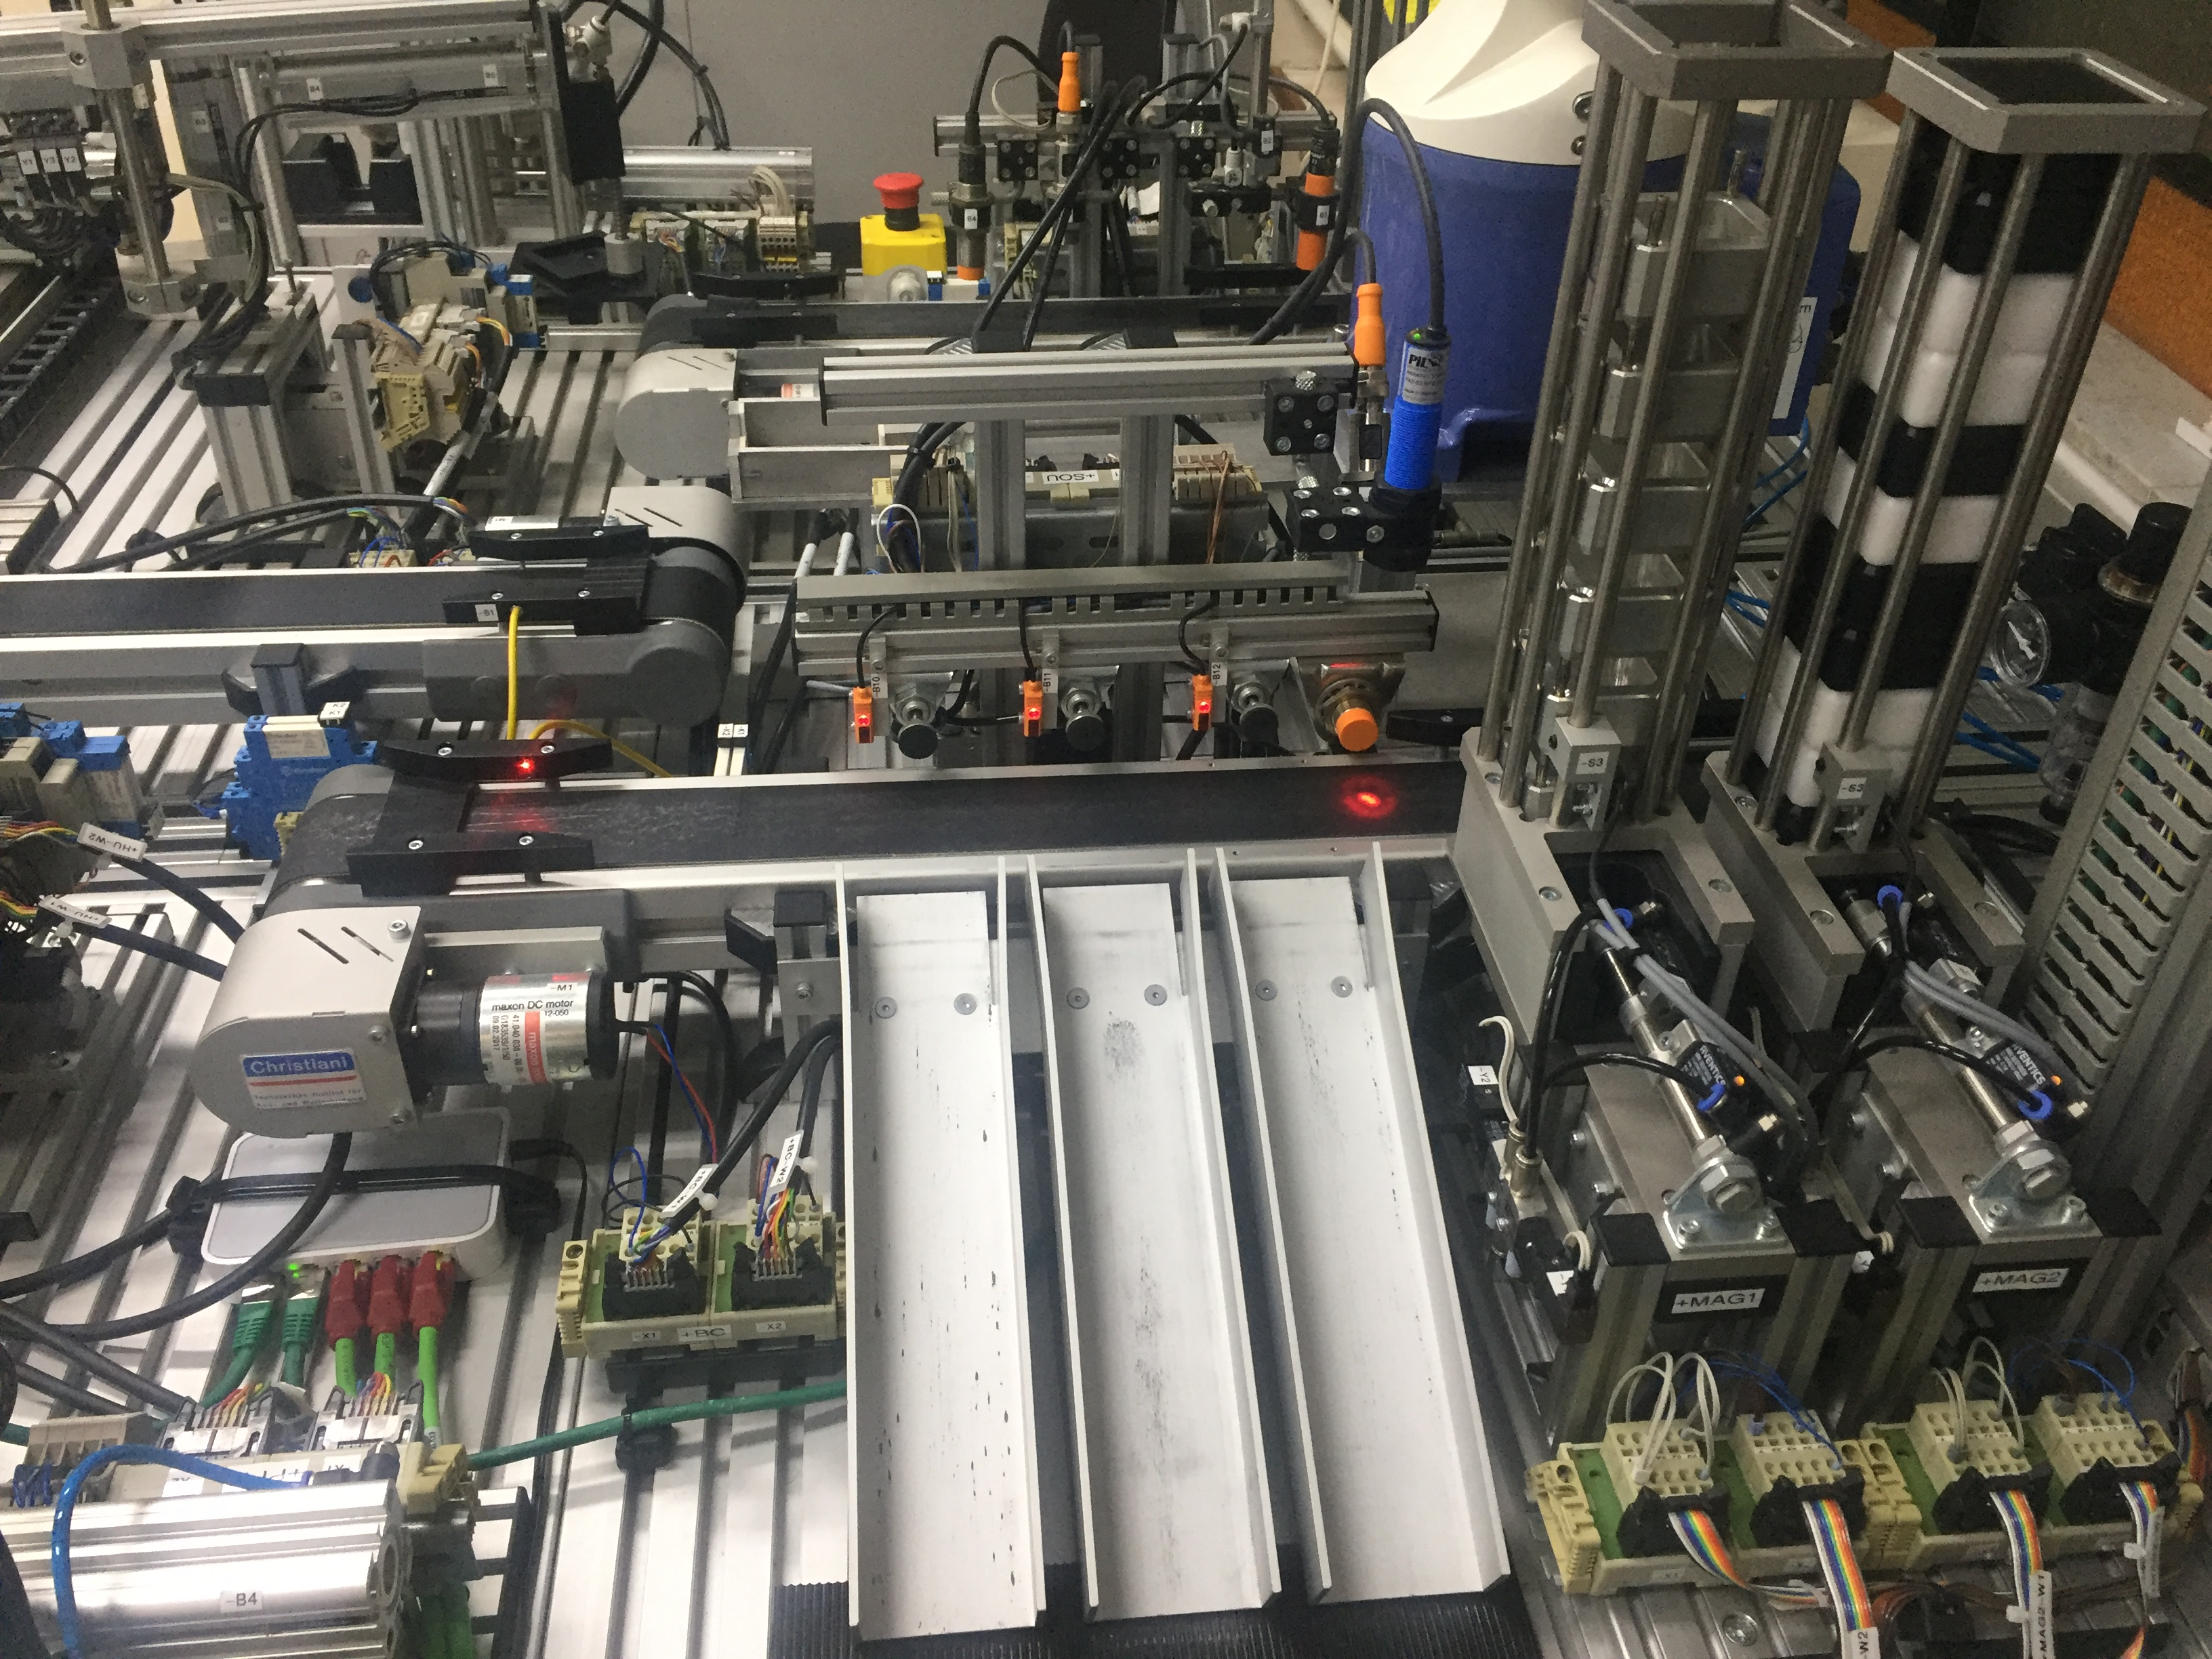
\includegraphics[width=6cm]{IMG_2206}}{IMG_2204.mov}
	\end{center}
	\begin{center}
		\movie[externalviewer]{\underline{Rede de Petri interpretada}}{rpic_planta.pdf}
	\end{center}
\end{block}

\end{frame}

\begin{frame}{Modelo do sistema}
	\begin{block}{Sinais do controlador}
		\begin{itemize}
			\item Vetor I/O composto por 23 sinais binários
			\begin{itemize}
				\item 15 de saída
				\item 8 de entrada
			\end{itemize}
		\end{itemize}
	\end{block}
	\begin{block}{Caminhos}
		\begin{itemize}
			\item 3533 caminhos observados
			\item 64 caminhos com intervalos de tempo (usando 1º método)
		\end{itemize}
	\end{block}
	\begin{block}{Modelo obtido com $ k = 1 $}
		\begin{itemize}
		\item 30 estados
		\item 64 caminhos
		\end{itemize}
	\end{block}
\end{frame}

\begin{frame}{Análise do modelo}
	\begin{block}{Primeira transição do caminho 6}
		\begin{figure}
			\centering
			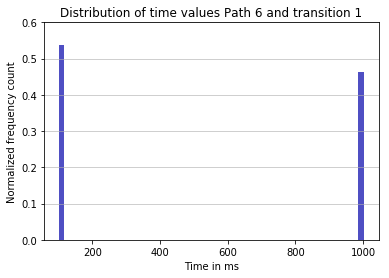
\includegraphics[width=8cm]{dist_timeValues}
%			\caption{Distribuição dos valores de tempo para a primeira transição do caminho com intervalos de tempo $ p_6' $.}
%			\label{fig:dist time values}
		\end{figure}  
	\end{block}
\end{frame}

\begin{frame}{Análise do modelo}
	\begin{block}{Parte do autômato obtido}
		\begin{figure}
			\centering
			\begin{tikzpicture}[shorten >=1pt,node distance=2cm,on grid,auto] 
			\node[state,accepting] (x0) [xshift=-2cm]  {$0$}; 
			\node[state] (x5) [right=of x0,xshift=3cm] {$5$};
			\node[state] (x24) [below=of x5] {$24$};
			\node[state] (x8) [above=of x5,yshift=1cm] {$8$};
			\node[state] (x25) [right=of x5,xshift=0.6cm] {$25$};
			
			\path[->] 
			(x0) edge  node {\scriptsize$ \begin{array}{c}
				\text{[101,104]} \\
				\cup \\
				\text{[1001,1003]} 
				\end{array} $} (x5)
			(x5) edge  node {$ [514,537]  $} (x25)
			(x5) edge [bend right] node [anchor=west]{$ [4052,4132] $} (x8)
			(x8) edge [bend right] node [anchor=east]{$ [914,939] $} (x5)
			(x5) edge [bend right] node [anchor=east]{$ [529,552] $} (x24)
			(x24) edge [bend right] node [anchor=west]{$ [909,935] $} (x5)
			;
			%\draw[fill=black] (2.5,0.5cm) circle (0.1cm);
			\draw[->] (-2.8,0) -- (-2.5,0);
			%\draw[->] (x3) to[out=-130,in=-40] node[pos=0.5,below]{\scriptsize$ a,\!\left\lbrace 2:I_{2,2} \right\rbrace $} (x2) ;
			\end{tikzpicture}
%			\caption{Parte do modelo TAOCT obtido para o sistema em que são apenas mostrados os estados e as transições envolvidos no caminho 6.}
%			\label{fig:practical} 
		\end{figure}
	\end{block}
\end{frame}

\section{Conclusões}

\begin{frame}{Conclusões}
	\begin{block}{}
		\begin{itemize}
			\item Apresentação da modelagem por identificação
			\item Proposta de um modelo temporizado
			\item Maior capacidade de detecção de falhas usando o modelo proposto
		\end{itemize}
	\end{block}
	\begin{block}{Trabalhos futuros}
		\begin{itemize}
			\item Estratégia de detecção de falhas explorando as vantagens do modelo proposto
			\item Isolamento das falhas detectadas
		\end{itemize}
	\end{block}
\end{frame}

\begin{frame}
\Large{MUITO OBRIGADO A TODOS!}
\begin{center}
\begin{itemize}
\item contato: ryanpitanga@poli.ufrj.br
\end{itemize}
\end{center}
\end{frame}

%\begin{frame}{Exemplo de 2 figuras}
%\begin{block}{} % Mesmo que o bloco não tenha título, coloque {}
%	\begin{figure}
%		\begin{center}
%			\begin{tabular}{cc}
%				
\includegraphics[width=4cm]{minerva_01.pdf}  & 
\includegraphics[width=3.5cm]{minerva_02.jpg}  \\
%				Minerva 1 & Minerva 2  % The printed column width is 8.4 cm.
%			\end{tabular}
%		\end{center}
%	\end{figure}
%	
%\end{block}
%\end{frame}



\end{document}





